\section{CLUSTERING}
The goal of our project is to do clustering based on variables except for \textbf{Weight} and \textbf{Height}, in order to find whether there are some relationships between those features and obesity levels. 
\subsection{Data Pre-processing}
All of those categorical data and obesity levels in the raw dataset are presented by the text, for simplicity, we set integer values instead of them: \textbf{Gender}(0:Female/1:Male), \textbf{family history with overweight}(0: No/1: Yes),\textbf{ FAVC}: Frequent consumption of high-caloric food (0: No/1: Yes), \textbf{CAEC}: Consumption of food between meals(0: no/1: sometimes/2: frequently/3: always), \textbf{SMOKE} (0: No/1: Yes), \textbf{SCC}: Calories consumption monitoring(0: No/1: Yes), \textbf{CALC}:Consumption of alcohol(0: no/1: sometimes/2: frequently/3: always), \textbf{MTRANS}: Transportation used (0: Walking/1: Bike/2: Motorbike/3: Public Transportation/4: Automobile), \textbf{NObeyesdad}: Obesity level (1: Insufficient Weight, 2: Normal Weight, 3: Overweight Level I, 4: Overweight Level II, 5: Obesity Type I, 6: Obesity Type II and 7: Obesity Type III)

\subsubsection{Numeric Data Analysis}
To separate observations into groups, a notion of dissimilarity between any two observations has to be defined. Euclidean distance is one of the most popular measurements to help us measure how similar two observations are, however, for observations with categorical variables, Euclidean distance is not sensible. In \ref{dis_sec}, we introduce another distance that is suitable for dealing with mixed data types. Since this measurement is sensitive to non-normality\cite{brown2012testing} in continuous variables, an analysis for normality of continuous data is necessary.
\begin{table}[!h]
\begin{center}
\begin{tabular}{ c| c | c |c |c |c |c }
\hline
    NAME  & Age & FCVC & NCP & CH2O & FAF & TUE \\
    \hline
 Skewness & 1.5280136 & -0.4325982 & -1.1063104& -0.1048371 & 0.4981353 & 0.6180628 \\
 \hline
\end{tabular}
\caption{\label{skew}Skewness of continuous variables}
\end{center}
\end{table}

Table \ref{skew} shows that \textbf{Age} has positive skewness, while \textbf{NCP} has negative skewness. To fix the non-normality, we set 
\begin{align}
    \textbf{Age} &<- \log_{10}(\textbf{Age})\notag \\ 
    \textbf{NCP} &<-\log_{10}(max(\textbf{NCP}+1)-\textbf{NCP})\notag
\end{align}

After the logistic transformation, the skewness of \textbf{Age} is 0.8671199 and that for \textbf{NCP} is 0.2019099.

\subsubsection{Gower Distance}\label{dis_sec}

Here, we introduce Gower distance\cite{gower1971general} to construct the dissimilarity matrix for mixed sorts of data. Gower distance can be used to measure the difference between any pairs in mixed types of data, including numerical, categorical, logical, and text data. The greater the Gower distance, which ranges from 0 to 1, the more unlike the two observations are from one another. For a quick check, we print out the most similar pair and the most dissimilar pair, or the pair with the least and maximum Gower distances. As shown in Table \ref{t2}, Ob1 and Ob2 are both males, they have the same lifestyle, and similar age, both of them have a family history of being overweight, and they also have the same level of obesity: Obesity Type I.Ob3 and Ob4 are the most dissimilar pair; one is very young and the other is considerably older; both do not smoke, however, their other habits are significantly different.
\begin{table}[!h]
\begin{center}
\scalebox{0.8}{
\begin{tabular}{ c | c c c c c c c c}
\hline
 \multicolumn{9}{c}{the most similar pair} \\
 \hline
      & Gender & Age & FhisW& FAVC & FCVC & NCP & CAEC & SMOKE \\
    \hline
Ob1 & 1 &	23.32934&	1&	1&	2&	3&	1&	0\\
Ob2 & 1&	23.32471&	1&	1&	2&	3&	1&	0\\
\hline
& CH2O & SCC & FAF & TUE & CALC & MTRANS & NObeyesdad &  \\
\hline
Ob1 &	3&	0&	3&	2&	0&	3&	5\\
Ob2 &	3&	0&	3&	2&	0&	3&	5 \\
  \hline
  \multicolumn{9}{c}{the most different pair} \\
 \hline
     & Gender & Age & FhisW& FAVC & FCVC & NCP & CAEC & SMOKE \\
    \hline
 Ob3 & 0	& 18.53084 &	0 & 	1&	1.21498	&1.717608&	1	&0\\
 Ob4  & 1&	55.00000&	1&	0&	3.00000	&4.000000&	2&	0\\
 \hline
 & CH2O & SCC & FAF & TUE & CALC & MTRANS & NObeyesdad &  \\
\hline
Ob3 &	1.179942	&0	&0.684739	&2&	1&	3&	1 \\
Ob4 &3.000000&	1&	3.000000&	0	&2&	0&	3\\ 
\end{tabular}
}
\caption{\label{t2} Two pairs of observations in dataset. FhisW: family history of Overweight}
\end{center}
\end{table}


\subsection{Hierarchical Clustering}

With Gower distance, we can do clustering then. In this section, we discuss hierarchical clustering. There are two primary categories of hierarchical clustering: divisive and agglomerative, the former acts top-down while the latter operates bottom-up. As a result, divisive hierarchical clustering is good for identifying large clusters, whereas agglomerative clustering is good for identifying small clusters\cite{bridges1966hierarchical}. Conducting those methods with Gower distance, we obtained plots as follows.

\begin{figure}[!htb]
   \begin{minipage}{1\textwidth}
     \centering
     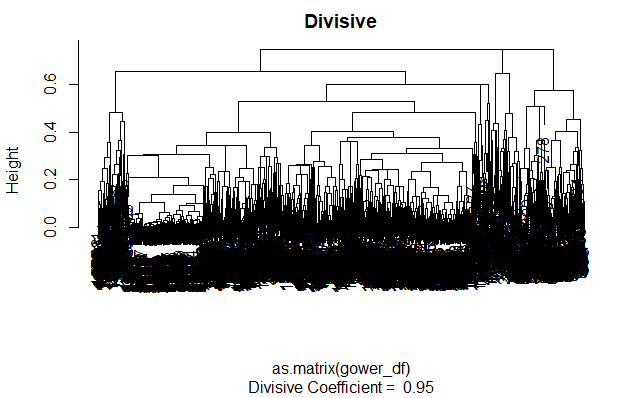
\includegraphics[width=1\linewidth]{image/hir_div.png}
     \caption{Divisive Hierarchical Clustering}\label{hir_div}
   \end{minipage}\hfill
   \\
   \begin{minipage}{1\textwidth}
     \centering
     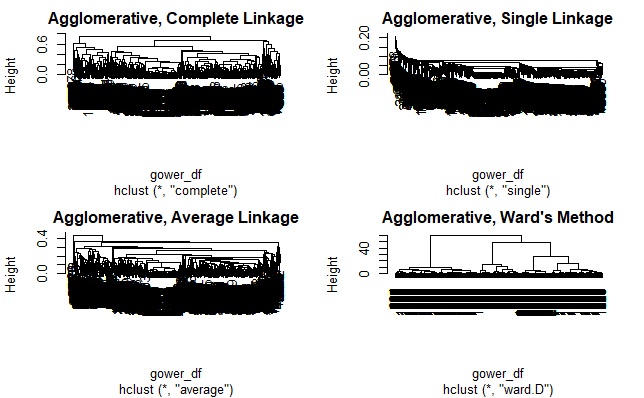
\includegraphics[width=1\linewidth]{image/hir_agg.png}
     \caption{Agglomerative Hierarchical Clustering}\label{hir_agg}
   \end{minipage}
\end{figure}

Since our dataset is balanced, we anticipate that the number of observations in each cluster will be close to average. The plots of divisive clustering and agglomerative clustering with complete linkage and Ward's methods appear to meet our expectations. In the following section, we will look at these three results.

\subsubsection{Optimal number of clusters}

The goal of clustering is to minimize dissimilarity within groups while maximizing the distance between groups, while also determining an appropriate number of clusters. It is critical to determine the optimal number of clusters. Here are two methods for us to consider; however, not both are appropriate for our situation\cite{reusova2018hierarchical}. In the project, we applied both of them on our clustering models, trying to find the most satisfactory result\\

The first is the Elbow method, which is based on the sum of squares within clusters. The observations inside the clusters are closer as it gets lower. Since we don't want too many clusters and the sum of squares would fall as the number of clusters increased, we would like to select the "elbow point," where further splitting of clusters results in just a slight reduction in the sum of squares. According to Figure \ref{elb}, we would like to choose 9 clusters for divisive model, 7 for agglomerative clustering with completed linkage and ward's method. Though the line in the third plot is smooth, 7 is still a sensible point, because the sum of square here is small enough compare with the first two plots.\\
However, after cutting hierarchical trees respectively, we had Table \ref{t3}. We can find that there are some clusters that have a small size in both the divisive model and agglomerative model with completed linkage, while the result of the agglomerative model with the Ward's method seems better. 

\begin{table}[!h]
\begin{center}
\begin{tabular}{ c | c c c c c c c c c}
\hline 
& 1& 2 & 3& 4& 5& 6& 7 & 8 & 9\\
\hline
Div & 117 & 37&  91& 110 &695 &833 & 31& 171 &  26 \\
Agg_c & 129 & 13 &371 &719& 837 & 37  & 5 & & \\
Agg_w & 128 & 79 & 142 & 381  & 854 & 205 & 322 \\
\end{tabular}
\caption{\label{t3} Number of observations in each clusters}
\end{center}
\end{table}

\begin{figure}[!htb]
   \begin{minipage}{0.8\textwidth}
     \centering
     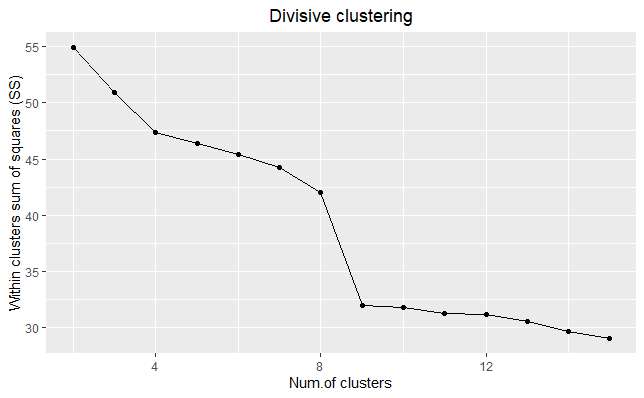
\includegraphics[width=1\linewidth]{image/elb_div.png}
   \end{minipage}\hfill
   \begin{minipage}{0.8\textwidth}
     \centering
     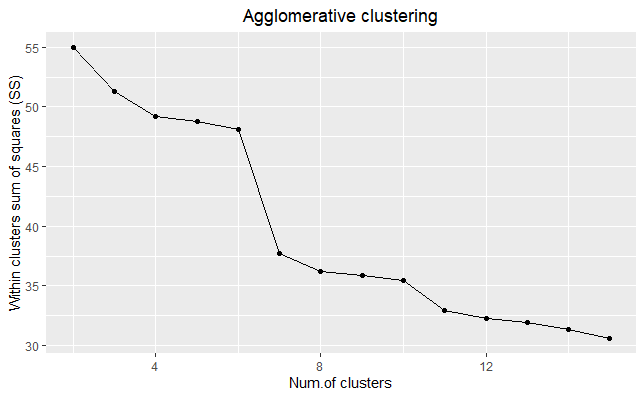
\includegraphics[width=1\linewidth]{image/elb_agg_c.png}
   \end{minipage}
   \begin{minipage}{0.8\textwidth}
     \centering
     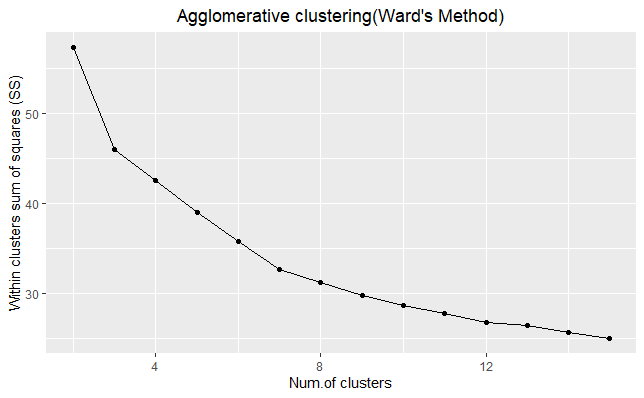
\includegraphics[width=1\linewidth]{image/elb_agg_w.png}
   \end{minipage}
   \caption{Elbow method}\label{elb}
\end{figure}

The second method is Silhouette method. In this case, we need to maximize the silhouette coefficient, as we want clusters that are distinctive enough to be considered separate. According to Figure \ref{sil}, this method is not that appropriate for the first two clustering model, as the point could be selected would be either too small or too large. However, for agglomerative clustering with Ward's method, the plot suggests us to choose 7 clusters, which is consistent with the result of elbow method. Therefore, we select it as our final model.

\begin{figure}[!htb]
   \begin{minipage}{0.8\textwidth}
     \centering
     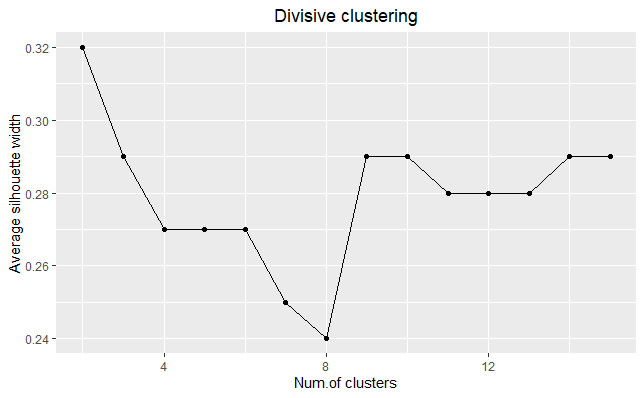
\includegraphics[width=1\linewidth]{image/shi_div.png}
   \end{minipage}\hfill
   \begin{minipage}{0.8\textwidth}
     \centering
     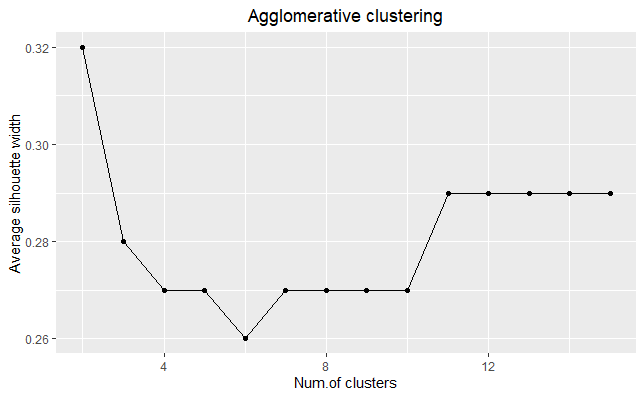
\includegraphics[width=1\linewidth]{image/shi_agg_c.png}
   \end{minipage}
   \begin{minipage}{0.8\textwidth}
     \centering
     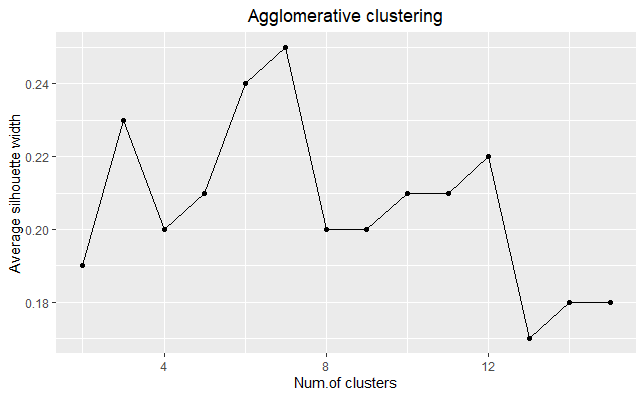
\includegraphics[width=1\linewidth]{image/shi_agg_w.png}
   \end{minipage}
   \caption{Silhouette method}\label{sil}
\end{figure}



\subsection{Partitioning Around Medoids Clustering}

In this section, we will discuss the Partitioning Around Medoids Clustering(PAM). PAM is an iterative clustering method similar to K-means, but it iterates repeatedly until the medoids don't move, replacing the centroids in K-means clustering. A member of a cluster who represents the median of all the factors being taken into account is called a medoid. In this project, we operate PAM with Gower distance.

A decided number of clusters is required before we conduct PAM, we use the Silhouette method here. Figure \ref{sil_pam} suggests 5 cluster is optimal. One of the advantages of PAM is that we can get the information of each group's medoid\ref{med}, thus getting the properties of each group. The medoid of a group can represent other members of the group to some extent. Considering the fourth group, we can see that the medoid's obesity level is insufficient weight, and other feature shows that she is a female, without a family history of overweight FAF(physical activity frequency) and NCP( number of main meals) are lower than other medoids, those features all make sense. While the only other medoid without a family history of being overweight is the third one, we can see he is of normal weight, and frequently does physical activity.\\
From the table, we can see that the medoids of the 5 groups are labeled with different obesity levels, which is really meaningful for us to explore the relationship between those features and the level of obesity.
\begin{figure}
    \centering
    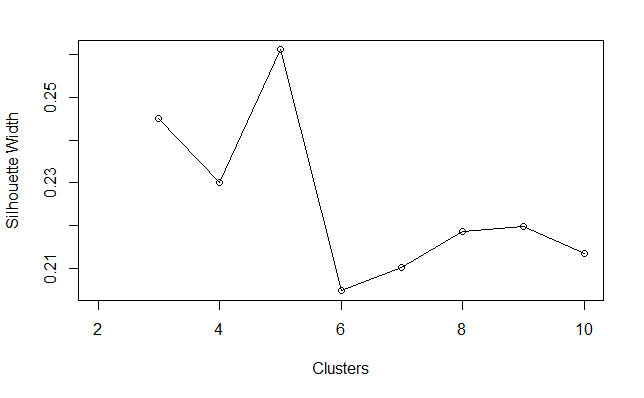
\includegraphics[width=1\linewidth]{image/shi_pam.png}
    \caption{Silhouette method for PAM}
    \label{sil_pam}
\end{figure}

\begin{figure}[!htb]
   \begin{minipage}{1\textwidth}
     \centering
     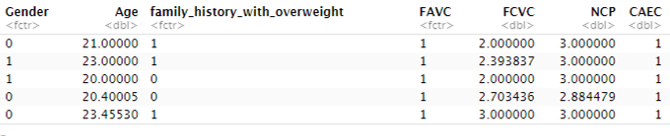
\includegraphics[width=1\linewidth]{image/Picture1.png}
   \end{minipage}\hfill
   \\
   \begin{minipage}{1\textwidth}
     \centering
     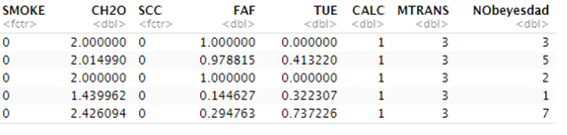
\includegraphics[width=1\linewidth]{image/Picture2.png}
   \end{minipage}
   \caption{Medoids}\label{med}
\end{figure}


